\section{Unsupervised learning}
In unsupervised learning one is given $N$ observations $x_1, x_N$ of a random $p$-vector $X$ having joint density $Pr(X)$. The goal is to directly infer the properties of this probability density without the help of a supervisor providing correct answers or degree of error. 

The dimension of $X$ is sometimes much higher than in supervised learning, and the properties of interest are often more complicated than simple location estimates. These factors are somewhat mitigated by the fact that $X$ represents all of the variables under consideration; one is not required to infer how the properties of $Pr(X)$ change, conditioned on the changing values of another set of variables.

In the context of unsupervised learning, there is no such direct measure of success. It is difficult to ascertain the validity of inferences drawn from the output of most unsupervised learning algorithms. One must resort to heuristic arguments not only for motivating the algorithms, as is often the case in supervised learning as well, but also for judgements as to the quality of the results. 

\subsection{Association rule}
The goal is to find joint values of the variables $X = (X_1, X_2, \cdots , X_p)$ that appear most frequently in the data base. It is mostly applied to binary-valued data $X_j = \{0,1\}$, where it is referred to as \textbf{Market basket analysis}. n this context the observations are sales transactions, such as those occurring at the checkout counter of a store. The variables represent all of the items sold in the store. For observation i, each variable $X_j$ is assigned $1$ if the item is purchased, $0$ otherwise.

More generally, the basic goal of association rule analysis is to find a collection of prototype $X$-values $v_1,\cdots,v_L$ for the feature vector $X$, such that the probability density $Pr(v_\ell)$ evaluated at each of those values is relatively large. This basically means find any kind of pattern that tells us how things go together. In this way the problem can be seen as \textbf{mode finding} or \textbf{bump hunting}.

A natural estimation of $Pr(v_\ell)$ is the number of occurrences for which $X=v_\ell$. With a large number of variables however, such observations will be to few to be reliable. The problem can be restated in another way.

Instead of seeking the values $x$ where $Pr(x)$ is large, one seeks region of the $X$-space with high probability content relative to their size or support.
\begin{definition}{\textbf{Support}}
The support $\CMcal{S_j}$ of a variable $j$is the set of all possible values for the variable.
\end{definition}
Let $\CMcal{S_j}$ represent the set of all possible values of the $j-th$ variable (its support) and let $ s_j \subseteq \CMcal{S_j}$ be a subset of these values. The modified goal can be stated as attempting to find subsets of variable values $s_1, \cdots, s_p$ such that the probability of each of the  variables is simultaneously assuming a value within its respective subset

\begin{equation}
Pr\left[ \bigcap\limits_{j = 1}^p \br{X_j \in s_j}\right]
\end{equation}
 is relatively large. $\bigcap\limits_{j = 1}^p \br{X_j \in s_j}$ is the intersection of subsets and it is called \textbf{conjunctive rule}.

\subsubsection{Market basket analysis}
For commercial databases $p\sim 10^4$, $N \sim 10^8$. In this cases many existing algorithm are not feasible and market basket analysis is applied.

Some simplifications are required: either $s_j$ consists of a single value of $X_j$ ($s_j = v_{0j}$), or it consists of the entire set of values of $X_j$ ($s_j = S_j$). So this simplifies to the problem of identifying the subset for which $s_j$ is a single value and and this  set is named $\CMcal{J} \subset \{1,\cdots,p\}$ and for each element in this subset find the corresponding value $v_{0j}$ such that:
\begin{equation}
Pr\left[ \bigcap\limits_{j \in \CMcal{J}} \br{X_j = v_{0j}}\right]
\label{dummyVarProb}
\end{equation}
is large.

One can apply the technique of dummy variables to turn \autoref{dummyVarProb} into a problem involving only binary-valued variables. Here we assume that the support $S_j$ is finite for each variable $X_j$. Specifically, a new set of variables $Z_1, \cdots, Z_K$ is created, one such variable for each of the values $v_{lj}$ attainable by each of the original variables $X_1, \cdots, X_p$. The number of dummy variables $K$ is
\begin{equation}
K = \sum_{j=1}^p |\CMcal{S}_j|
\end{equation}
where $|\CMcal{S}_j|$ is the number of distinct values attainable by $X_j$.  Each dummy variable is assigned the value $Z_k = 1$ (with $Z_k$ being associated to $v_{lj}$), if the variable with which it is associated takes on the corresponding value to which $Z_k$ is assigned (i.e., $Z_k$ is associated with $v_{lj}$; $Z_k = 1$ if  $X_j=v_{lj}$), and $Z_k = 0$ otherwise. This corresponds to find a subset of integers $\CMcal{K} \subset \{1,\cdots, K\}$ such that:

\begin{equation}
Pr\left[ \bigcap\limits_{k \in \CMcal{K}} \br{Z_k = 1}\right] = Pr\left[ \prod_{k \in \CMcal{K}} Z_k = 1\right]
\end{equation}
is large.

This is the standard formulation of the market basket problem. The set $K$ is called an \textbf{item set}. The number of variables $Z_k$ in the item set is called its "size" (note that the size is no bigger than $p$).

The estimated value of the previous expression is taken to be the fraction of observations in the database for which the conjunction is true:
\begin{equation}
\hat{Pr}\left[ \bigcap\limits_{k \in \CMcal{K}} \br{Z_k = 1}\right] = \frac{1}{N}\sum_{i=1}^N \prod_{k \in \CMcal{K}} z_{ik}
\end{equation}
where $z_{ik}$ is the value of $Z_k$ in the $i$-th case. This is called support or prevalence $T(\CMcal{K})$ if the item-set $\CMcal{K}$.

In association rule, a lower support bound $t$ is specified and one seeks all sets $\CMcal{K}_\ell$ that can be formed from the variables $Z_k$ with support in the data base greater than this lower bound $t$.

\subsubsection{Apriori algorithm}
For a given support threshold $t$ The cardinality $|\{\CMcal{K}| T(\CMcal{K}) \}|$ is relatively small. Any item set consisting of a subset of the items $\CMcal{K}$ must have support greater than or equal to that of  $\CMcal{K}$:  $\CMcal{L} \subseteq \CMcal{K} \Rightarrow T(\CMcal{L})\ge T(\CMcal{K})$.

The first pass over the data computes the support of all single-item sets. Those whose support is less than the threshold are discarded. The second pass computes the support of all item sets of size two that can be formed from pairs of the single items surviving the first pass. Each successive pass over the data considers only those item sets that can be formed by combining those that survived the previous pass with those retained from the first pass. Passes over the data continue until all candidate rules from the previous pass have support less than the specified threshold.

The items $Z_k$, $k \in K$, are partitioned into two disjoint subsets, $A \cup B = K$, and written $A\Rightarrow B$. $A$ is called antecedent and $B$ consequent.

Association rules are defined to have several properties based on the prevalence of the antecedent and consequent item sets in the data base. The support of the rule $T(A\Rightarrow B)$ is the fraction of observations in the union of the antecedent and consequent, which is just the support of the item set $K$ from which they were derived. It can be viewed as an estimate of the probability of simultaneously observing both item sets $Pr(A \text{and} B)$ in a randomly selected market basket. The "confidence" or "predictability" $C(A\Rightarrow B)$ of the rule is its support divided by the support of the antecedent:
\begin{equation}
C(A\Rightarrow B) = \frac{T(A\Rightarrow B)}{T(A)}
\end{equation}
which can be viewed as an estimate $Pr(A|B)$.

The "expected confidence" is defined as the support of the consequent $T(B$), which is an estimate of the unconditional probability $Pr(B)$. Finally, the "lift" of the rule is defined as the confidence divided by the expected confidence:
\begin{equation}
L(A\Rightarrow B) = \frac{C(A\Rightarrow B)}{T(B)}
\end{equation}
This is an estimate of the association measure $Pr(A \text{and} B)/Pr(A)Pr(B)$.

Suppose the item set $K = \{peanut butter, jelly, bread\}$ and consider the rule $\{peanut butter, jelly\} \Rightarrow \{bread\}$. A support value of $0.03$ for this rule means that peanut butter, jelly, and bread appeared together in $3\%$ of the market baskets. A confidence of $0.82$ for this rule implies that when peanut butter and jelly were purchased, $82\%$ of the time bread was also purchased. If bread appeared in $43\%$ of all market baskets then the rule $\{peanut butter, jelly\} \Rightarrow \{bread\}$ would have a lift of $1.95$.

A confidence threshold c is set, and all rules that can be formed from those item sets with confidence greater than this value:
\begin{equation}
\{ A\Rightarrow B| C(A\Rightarrow B)>c\}
\end{equation}


The output of the entire analysis is a collection of association rules (14.7) that satisfy the constraints:
\begin{equation}
T(A \Rightarrow B) >t \quad \text{and}\quad C(A \Rightarrow B)>c
\end{equation}

\subsection{Generalized association rule}
...

\subsection{Cluster Analysis}
The goal is grouping or segmenting a collection of objects into subsets or "clusters", such that those within each cluster are more closely related to one another than objects assigned to different clusters. Objects can be described by a set of measurements, or by relations to other objects. In addition, the goal is sometimes to arrange the clusters into a natural hierarchy. This involves successively grouping the clusters themselves.

A clustering method attempts to group the objects based on the definition of similarity supplied to it.

K-means clustering starts with guesses for the three cluster centers. Then it alternates the following steps until convergence:
\begin{itemize}
\item  for each data point, the closest cluster centre (in Euclidean distance) is identified;
\item each cluster centre is replaced by the coordinate-wise average of all data points that are closest to it.
\end{itemize}

This is a top-down procedure.

\subsubsection{Proximity Matrices and dissimilarities}
In social science experiments, participants are asked to judge by how much certain objects differ from one another. Dissimilarities can then be computed by averaging over the collection of such judgements.

This type of data can be represented by an $N \times N$ matrix $D$, where $N$ is the number of objects, and each element $d_{ii'}$ records the proximity between the $i$-th and $i'$-th objects. Most algorithms use $d_{ii}= 0$ and non negative weights.

Some algorithms require a dissimilarity matrix. Given $d_j(x_{ij}, x_{i'j}$ a dissimilarity between values of the $j$-the attribute, we define the dissimilarity between objects $i$ and $i'$ as:
\begin{equation}
D(x_i, x_{i'}) = \sum_{j=1}^p d_j (x_{ij}, x_{i'j})
\end{equation}
Most likely $d_j$ is the squared distance. For quantitative variables other common choice are the absolute error or correlation:
\begin{equation}
\rho(x_i, x_{i}) = \frac{\sum_j (x_{ij} - \bar{x}_i)(x_{i'j} - \bar{x}_i)}{\sqrt{\sum_j (x_{ij} - \bar{x}_i)^2(x_{i'j} - \bar{x}_i)^2}}
\end{equation}
\textbf{Ordinal variables} are often represented as contiguous integers. Examples are academic grades (A, B, C, D, E, F), degree of preference and so on. 
\textbf{Categorical or nominal variables} one can build a symmetric matrix with $M$ values s.t. $L_{ij}=L_{ji}\ge 0$ and $L_{ii}=0$. A popular choice is $L_{ii} = 0$.

To calculate \textbf{dissimilarity between objects} generally a weighted average is used:
\begin{equation}
D(x_i, x_{i'}) = \sum_{j=1}^p w_j d_j (x_{ij}, x_{i'j})
\end{equation}
Let us define the average dissimilarity on the $j$-th attrbute as:
\begin{equation}
\bar{d}_j = \frac{1}{N^2}\sum_{i=1}^N\sum_{i'=1}^N d_j(x_{ij}x_{i'j})
\end{equation}
We might define $w_j \sim \frac{1}{\bar{d}_j}$would give all attributes equal influence in characterizing overall dissimilarity between objects. In general, setting $w_j = \frac{1}{\bar{d}_j}$ for all attributes, irrespective of type, 
will cause each one of them to equally influence the overall dissimilarity between pairs of objects. However, if the goal is to segment the data into groups of similar objects, all attributes may not contribute equally to the (problem-dependent) notion of dissimilarity between objects.

\subsubsection{Combinatorial Algorithms}
Combinatorial algorithms work directly on the observed data with no direct reference to an underlying probability model. They assign each observation to a group or cluster without regard to a probability model describing the data. Each observation is uniquely labeled by an integer $i \in \{1,\cdots, N\}$.

A prespecified number of clusters $K<N$ is assumed.  Each observation is assigned to one and only one cluster. Given the dissimilarities between every pair of observations we want to assign each point to a cluster by the algorithm outputting a value corresponding to the cluster.

One approach is to directly specify a mathematical loss function and attempt to minimize it through some combinatorial optimization algorithm.Since the goal is to assign close points to the same cluster, a natural loss (or "energy") function would be:

\begin{equation}
W(C)  = \frac{1}{2}\sum_{k=1}^K \sum_{C(i) = k} \sum_{C(i') = k} d(x_i, x_{i'})
\end{equation}
where $C(i) = k$ is an encoder assigning someway the point $i$ to the class $k$.
This criterion characterizes the extent to which observations assigned to the same cluster tend to be close to one another.

$W(C)$ is referred to as \textbf{within-cluster point scatter} while 
\begin{equation}
B(C) =\frac{1}{2} \sum_{k=1}^K \sum_{C(i) = k} \sum_{C(i') \ne k} d(x_i, x_{i'}
\end{equation}
as the \textbf{between-cluster point scatter} and
\begin{equation}
T = \frac{1}{2} \sum_{i=1}^N \sum_{i'=1}^N d_{ii'} = W(C) + B(C) = const
\end{equation}
is the \textbf{total point scatter} which is a constant given the data. $B(C)$ tends to be large when observations assigned to different clusters are far apart.
So we have $W(C) = T - B(C) $ minimizing $W(C)$ is equivalent to maximizing $B(C)$.

Such optimization by complete enumeration is feasible only for very small data sets. The number of distinct assignments is
\begin{equation}
S(N,K) = \frac{1}{K!} \sum_{k=1}^K (-1)^{K-k} \binom{K}{k} k^N
\end{equation}
For example, $S(10, 4) = 34105$ which is still feasible, but $S(19,4) \approx 10^{10}$.  For this reason, practical clustering algorithms are able to examine only a very small fraction of all possible encoders $k = C(i)$. The goal is to identify a small subset that is likely to contain the optimal one, or at least a good suboptimal partition. Such feasible strategies are based on iterative greedy descent.

\subsubsection{K-means}
The $K$-means algorithm is one of the most popular iterative descent clustering methods. It is intended for situations in which all variables are of the quantitative type, and squared Euclidean distance.
The within-point scatter can be written as:
\begin{equation}
\begin{aligned}
&W(C) = \frac{1}{2}\sum_{k=1}^K \sum_{C(i) = k} \sum_{C(i') = k} |x_i - x_{i'}|^2= \sum_{k=1}^K N_k \sum_{C(i) = k}  |x_i - \bar{x}_{k}|^2\\
& N_k = \sum_{i=1}^N I(C(i) = k)
\end{aligned}
\end{equation}
where $\bar{x}_k$ is the mean vector associated with the $k$th-cluster. So the $N$ observations are assigned in a way such that within each cluster the average dissimilarity of the observations from the cluster mean is minimized.
\begin{algorithm}
For a given cluster assignment $C$, the total cluster variance is minimized w.r.t. $m_1, \cdots, m_K$, yielding the means of the currently assigned clusters\;
Given a current set of means the total cluster variance is minimized by assigning each observation to the closest cluster mean: $C(i) = \argmin{1\le k\le K}{|x_i-m_k|^2}$\;
Iterate the previous steps until assignment do not change.
\caption{K-means algorithm}
\end{algorithm}

\subsubsection{Gaussian Mixtures as Soft K-means Clustering}
The K-means clustering procedure is closely related to the EM algorithm for estimating a certain Gaussian mixture model. The E-step of the EM algorithm assigns "responsibilities" for each data point based in its relative density under each mixture component, while the M-step recomputes the component density parameters based on the current responsibilities. Suppose we specify K mixture components, each with a Gaussian density having scalar covariance matrix $\sigma^2\I$. Then the relative density under each mixture component is a monotone function of the Euclidean distance between the data point and the mixture centre. Hence in this setup EM is a "soft" version of K-means clustering, making probabilistic (rather than deterministic) assignments of points to cluster centres. With $\sigma^2 \rightarrow 0$  the models coincide.

\subsection{Vector quantization}
Used in image processing to compress images at a cost of loss in quality. VQ breaks the image into small blocks of pixels $2 \times 2$ for example. Suppose the image is $1024 \times 1024$ pixels, then we get $512\times 512$ blocks of four pixels, i.e. a vector in $\CMcal{R}^4$. A k-means clustering algorithm is run in this space.  Each block is approximated with its closest cluster, known as codeword. The bigger $K$ the less lossy is the compression, and it is big enough we can achieve a lossless compression. The clustering process is called the encoding step, and the collection of centroids is called the codebook. To name and identify the codebook entries approximating the blocks will require $\log_2(K)$ bits per block. We also need to supply the codebook itself, which is $K \times 4$ real numbers.

\subsubsection{K-medoids}
Squared Euclidean distance places the highest influence on the largest distances. This causes the procedure to lack robustness against outliers that produce very large distances.  In the most common form, centres for each cluster are restricted to be one of the observations assigned to the cluster.
\begin{algorithm}
For a given cluster assignment C find the observation in the cluster
minimizing total distance to other points in that cluster:
\begin{equation}
i_k^* = \argmin{\{i:C(i) = k\}} \sum_{C(i')=k}D(x_i, x_{i'})
\end{equation}
Then $m_k=x_{i_k^*}$, $k=1,\cdots, K$ are the current estimates of the cluster centres\;
Given a current set of clusters centres $\{m_1, \cdots, m_K\}$ minimize the total error by assigning each observation to the closest current cluster centre:
\begin{equation}
C(i) = \argmin{1\le k\le K}{D(x_i, m_k)}
\end{equation}\;
Iterate the previous steps until the assignment do not change.
\caption{K-medoids}
\end{algorithm}
This algorithm assumes attribute data, but the approach can also be applied to data described only by proximity matrices.

\subsubsection{Number of cluster}
Suggestions range from simple random selection to a deliberate strategy based on forward stepwise assignment. At each step a new centre $i_k$ is chosen to minimize the given criterion, given the centres $i_1, \cdots, i_{k-1}$ chosen at the previous steps. This continues for $K$ steps, thereby producing $K$ initial centres with which to begin the optimization algorithm.

For data segmentation $K$ is usually defined as part of the problem. For example, a company may employ $K$ sales people, and the goal is to partition a customer database into $K$ segments, one for each sales person, such that the customers assigned to each one are as similar as possible.

In other cases it must be estimated typically by examining the within-cluster dissimilarity $W_K$ as a function of the number of clusters $K$. Separate solutions are obtained for $K \in \{1, \cdots , K_{max}\}$. Generally $W_k$ decreases with increasing $K$, even when the criterion is evaluated on an independent test set.

\subsubsection{Hierarchical clustering}
Hierarchical clustering methods require the user to specify a measure of dissimilarity between (disjoint) groups of observations, based on the pairwise dissimilarities among the observations in the two groups. They produce hierarchical representations in which the clusters at each level of the hierarchy are created by merging clusters at the next lower level. At the lowest level, each cluster contains a single observation. At the highest level there is only one cluster containing all of the data.

Strategies for hierarchical clustering divide into two basic paradigms: agglomerative (bottom-up, ) and divisive (top-down).

In agglomerative methods, the pair chosen for merging consist of the two groups with the smallest intergroup dissimilarity. For divise-methods, the split is chosen to produce two new groups with the largest between-group dissimilarity. With both paradigms there are $N - 1$ levels in the hierarchy.

Recursive binary splitting/agglomeration can be represented by a rooted binary tree. 

\subsubsection{Agglomerative clustering}
Agglomerative clustering algorithms begin with every observation representing a singleton cluster. At each of the $N - 1$ steps the closest two (least dissimilar) clusters are merged into a single cluster, producing one less cluster at the next higher level. Therefore, a measure of dissimilarity between two clusters (groups of observations) must be defined.

Given two groups $G$ and $H$ and two observations $i \in G$, $i' \in H$ the pairwise observation dissimilarity between these two points is $d_{ii'}$. The dissimilarity bbtw $G$ and $H$ is computed from the set of all dissimilarities.

\textbf{Single linkage} agglomerative clustering takes the intergroup dissimilarity to be that of the closest (least dissimalar) pair:
\begin{equation}
D_{SL} = \min_{i \in G, i' \in H} d_{ii'}
\end{equation}
This is often called \textbf{nearest neighbour technique}. \textbf{Complete linkage} agglomerative clustering  takes the intergroup dissimilarity to be that of the furthest pair (most dissimilar pair):
\begin{equation}
d_{CL} (G,H) = \max_{i \in G, i' \in H} d_{ii'}
\end{equation}
\textbf{Group average} clustering uses the average:
\begin{equation}
d_{GA} = \frac{1}{N_GN_H}\sum_{i \in G}\sum_{i' \in H}
\end{equation}
where $N$ are the num. observations in each group. If the data dissimilarities exhibit a strong clustering tendency, with each of the clusters being compact and well separated from others, then all three methods produce similar results.

Single linkage only requires that a single dissimilarity be small for two groups to be considered close together, irrespective of the other observation dissimilarities between the groups. It will therefore have a tendency to combine, at relatively low thresholds, observations linked by a series of close intermediate observations. This phenomenon, referred to as \textbf{chaining}, is often considered a defect of the method.

Complete linkage represents the opposite extreme. Two groups $G$ and $H$ are considered close only if all of the observations in their union are relatively similar. It will tend to produce compact clusters with small diameters.
However, it can produce clusters that violate the "closeness" property. That is, observations assigned to a cluster can be much closer to members of other clusters than they are to some members of their own cluster.
Group average clustering represents a compromise between the two extremes of single and complete linkage. It attempts to produce relatively compact clusters that are relatively far apart. However, its results depend on the numerical scale on which the observation dissimilarities are measured.
\subsubsection{Divisive clustering}
The divisive paradigm can be employed by recursively applying any of the combinatorial methods such as K-means or K-medoids , with $K = 2$, to perform the splits at each iteration.

A better approach is by Smith et. al(1965). It begins by placing all observations in a single cluster $G$. It then chooses that observation whose average dissimilarity from all the other observations is largest. This observation forms the first member of a second cluster $H$. At each successive step that observation in $G$ whose average distance from those in $H$, minus that for the remaining observations in $G$ is largest, is transferred to $H$. This continues until the corresponding difference in averages becomes negative. That is, there are no longer any observations in $G$ that are, on average, closer to those in $H$.

\subsubsection{Self-organizing maps}
...

\subsection{Principal components, curves and surfaces}
The principal components of a set of data in $\CMcal{R}^p$ provide a sequence of best linear approximations to that data, of all ranks $q \le p$. Given the observations $x_1, \cdots, x_N$, the linear approximation is:
\begin{equation}
f(\lambda) = \mu  + \mathbf{V}_q\lambda
\end{equation}
where $\mathbf{V}_q$ is a $p\times q$ matrix with $q$ orthogonal unit vectors as columns, $\lambda$ a $q$ vector of parameters and $\mu$ a location vector in $\CMcal{R}^p$. This is a $p$ hyperplane. Fitting such a model corresponds to minimize the reconstruction error:
\begin{equation}
\min_{\mu, \{\lambda_i\}, \mathbf{V}_q} \sum_{i=1}^N \| x_i -\mu - \mathbf{V}_q\lambda_u \|^2
\end{equation}
We can partially optimize to obtain:
\begin{equation}
\begin{aligned}
\hat{\mu} &= \bar{x}\\
\hat{\lambda}_i &= \mathbf{V}_q^T (x_i - \bar{x})
\end{aligned}
\end{equation}
so we must find the matrix $\mathbf{V}_q$:
\begin{equation}
\min_{\mathbf{V}_q} \sum_{i=1}^N  \| \br{x_i - \bar{x}} -\mathbf{V}_q\mathbf{V}_q^T\br{x_i - \bar{x}}\|^2
\end{equation}
For convenience we assume $\bar{x}=0$, if not true then one replaces with $\tilde{x}_i = x_i = \bar{x}$.
The matrix
\begin{equation}
\mathbf{H}_q = \mathbf{V}_q \mathbf{V}_q^T
\end{equation}
is a projection matrix so that each point $x_i$ is mapped onto its rank-$q$ reconstruction $\mathbf{H}_q x_i$, the orthogonal projection of $x_i$ spanned by the columns $\mathbf{V}_q$.

Consider the matrix $\X = \br{\x_1^T, \cdots, \x_N^T}$ of the observations and perform the singular value decomposition:
\begin{equation}
\X = \mathbf{U}\mathbf{D}\mathbf{V}^T
\end{equation}

$\mathbf{U}$ is a $N\times p$ orthogonal matrix $\mathbf{U}^T\mathbf{U}=\I_p$ whose columns $\mathbf{u}_j$ are called \textbf{left singular vectors}. $\mathbf{V}$ is a $p\times p$ orthogonal matrix ($\mathbf{V}^T\mathbf{V}=\I_p$) with columns $\mathbf{v}_j$ called the \textbf{right singular vectors}. $\mathbf{D}$ is a diagonal $p\times p$ matrix with $d_1\ge d_2\ge \cdots\ge d_p\ge 0$ known as \textbf{singular values}. 

For each rank $q$, (i.e., the chosen dimensionality on which the observations are projected), the solution $\mathbf{V}_q$  consists of the first $q$ columns of $\mathbf{V}$. The columns $\mathbf{UD}$ are called the \textbf{principal components} of $\X$. The $N$ optimal $\hat{\lambda}_i$ are given by the first $q$ principal components (the $N$ rows of the $N \times q$ matrix $\mathbf{U}_q\mathbf{D}_q$.

\autoref{SVDex} shows the one-dimensional principal component line in a $\CMcal{R}^2$ input space ($p=2$, $q=1$). For each observation point $x_i$ there is a closest point on the line given by $u_{i1}d_1v_1$ where $v_1$ is the direction of the line ($v_1$ is $p=2$ dimensional vector). $\hat{\lambda}_1=d_{i1}d_1$ measures distance along the line from the origin.

\begin{figure}
\centering
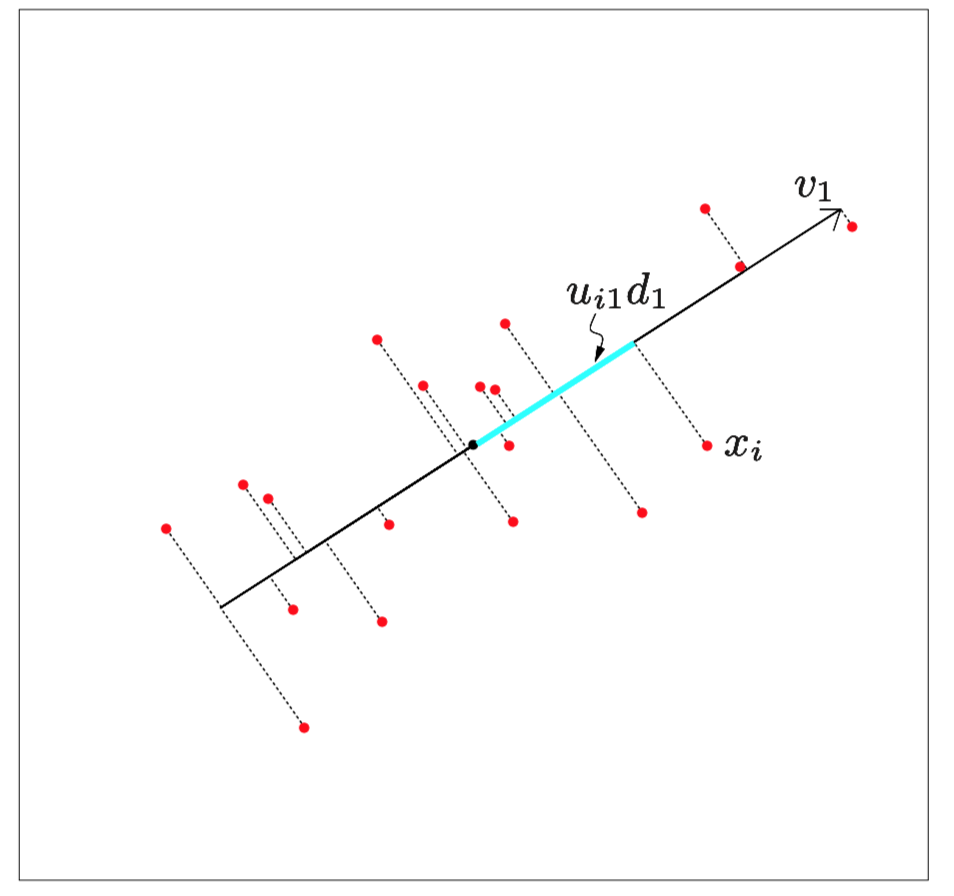
\includegraphics[scale=0.5]{img/SVD}
\caption{Example of SVD mapping of data from a $\CMcal{R}^2$ space (i.e., a plane) onto a line $\CMcal{R}$}
\label{SVDex}
\end{figure}
\subsubsection{Applications}
Principal components are a useful tool for dimension reduction and compression, for example for hand-written digits. If the inputs are $16\times 16$ images, inputs rely in  a $\CMcal{R}^{256}$ space.

\begin{figure}
\centering
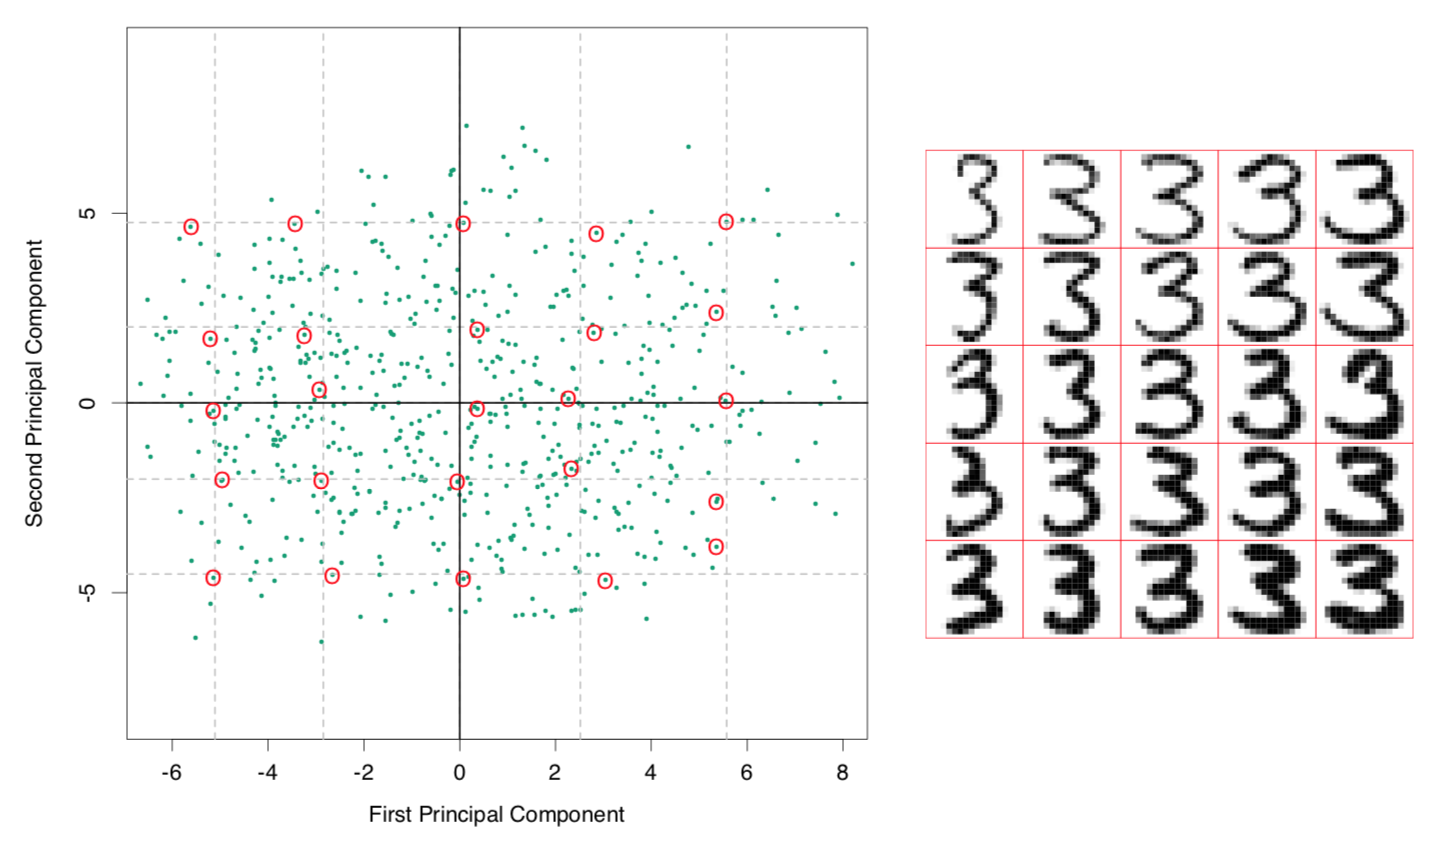
\includegraphics[scale=0.5]{img/2PC}
\caption{2 Principal components analysis applied on the $3$ hand-written digits.}
\label{2PC}
\end{figure}
Consider PCA on hand-written digits of a single number, for example a $3$, and perform two principal components analysis $u_{i1}d_1$ and $u_{i2}d_2$ of each observation and calculate the quantiles $5\%, 25\%, 50\% 75\%, 95\%$ indicated by the grid in \autoref{2PC}. Red circles indicate those images close to the vertices of the grid where distance is in terms of the projected coordinates (but some weight is given to the components in the orthogonal space (?)). On the right of \autoref{2PC} the images corresponding to the red circles are shown and this allows to visualize the nature of the first two PC. $v_1$, the horizontal direction, mainly accounts for the length of lower "tail" of the "$3$", $v_2$ the vertical axis  accounts for character thickness. The parametrized model is:
\begin{equation}
\hat{f}(\lambda) = \bar{x} + \lambda_1 v_1+\lambda_2 v_2 
\end{equation}
that in terms of images is something like the one in \autoref{modelImage}.


\begin{figure}
\centering
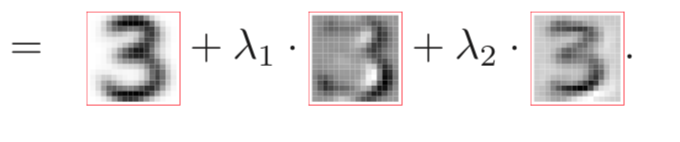
\includegraphics[scale=0.7]{img/modelImage}
\caption{Equivalence of the parametrized model using image representation.}
\label{modelImage}
\end{figure}
Although there are a possible 256 principal components, approximately 50 account for 90\% of the variation in the threes, 12 account for 63\%.

A relatively small subset of the principal components serve as excellent lower-dimensional features for representing the high-dimensional data.

The same technique, with some further calculations, can be applied to digital signature.

\subsubsection{Principal curves and surfaces}
Principal curves generalize the concept of the principal component line to obtain smoother curves. 

Let $f(\lambda)$ be a parametrized smooth curve in $\CMcal{R}^p$. It is a vector function of with $p$ coordinates, each a smooth function of the single parameter $\lambda$. For example $\lambda$ can be chosen to be the arc-length along the curve from a fixed origin. For each data value $x$, let $\lambda_f(x)$ define the closest point on the curve to $x$. Then $f(\lambda)$ is called a principal component curve for the distribution of the random vector $X$ if:
\begin{equation}
f(\lambda) = \E\br{X|\lambda_f(X) = \lambda}
\end{equation}
So $f(\lambda)$ is the average of all data points that project to it (\textbf{self-consistency} property). Although in practice, continuous multivariate distributes have infinitely many principal curves (Duchamp and Stuetzle, 1996), we are interested mainly in the smooth ones.

A principal curve is defined by its coordinate functions: $f(\lambda) =$ $[ f_1(\lambda), f_p(\lambda)]$ and let $X^T = (X_1, \cdots, X_p)$. Consider the following alternate steps:
\begin{equation}
\begin{aligned}
&1) \quad \hat{f}_j(\lambda)\leftarrow \E \br{X_j|\lambda(X) = \lambda}; \quad j=1,\cdots, p\\
&2) \quad \hat{\lambda}_f(x) \leftarrow \argmin{\lambda'}{\|x -\hat{f}(\lambda')\|^2}
\end{aligned}
\end{equation}
In the first $\lambda$ is fixed and it enforces the self-consistency requirement. In the second the curve is fixed and it finds the closest point on the curve to each data point.

With finite data, the principal curve algorithm starts with the linear principal component, and iterates the two steps until convergence.
A scatterplot smoother is used to estimate the conditional expectations in the frist step by smoothing each $X_j$ as a function of the arc-length $\lambda(X)$, and the projection in the second step is done for each of the observed data points. Proving convergence in general is difficult, but one can show that if a linear least squares fit is used for the scatterplot smoothing, then the procedure converges to the first linear principal component, and is equivalent to the power method for finding the largest eigenvector of a matrix.

Principal surfaces have exactly the same form as principal curves, but are of higher dimension. The mostly commonly used is the two-dimensional principal surface, with coordinate functions
\begin{equation}
f(\lambda_1, \lambda_2) = \left[ f_1(\lambda_1, \lambda_2), \cdots, f_p(\lambda_1, \lambda_2)\right]
\end{equation}
Principal surfaces of dimension greater than two are rarely used, since the visualization aspect is less attractive, as is smoothing in high dimensions.

\subsubsection{Spectral Clustering}
Traditional clustering methods like K-means use a spherical or elliptical metric to group data points. Hence they will not work well when the clusters are non-convex, such as the concentric circles.

Spectral clustering solves this problem by firstly building a $N\times N$ matrix of pairwise similarities $s_{ij}\ge 0$ between all observation pairs.We represent the observations in an undirected similarity graph $G = \left\langle V, E\right\rangle$. The $N$ vertices $v_i$ are the observations and pairs of vertices are connected by an edge if their similarity is positive or exceeds some threshold. Edges are weighted by $s_{ij}$.

Clustering now is a graph-partition problem where we identify connected components with clusters. We  want to partition the graph such that edges between different groups have low weight and within a group have high weight.

Consider $N$ points $x_i \in \CMcal{R}^p$ and let $d_{ij}$ be the Euclidean distance between $x_i$ and $x_j$. We will use as similarity matrix the radial-kernel matrix:
\begin{equation}
s_{ij} = \e^{-\frac{d_{ij}^2}{c}}
\end{equation}
where $c >0$ is a scale parameter. A popular way to define the similarity matrix is the \textbf{mutual K-nearest-neighbour graph}. Define $\mathcal{N}_k$ the symmetric set of nearby pairs of points: a pair $(i,j)$ is in $\mathcal{N}_k$ if $i$ is in the $K$-neighbourhood of $j$ or viceversa. Then we connect all NN and give them edge-weight $w_{ij} = s_{ij}$, otherwise the weight is $0$.
Alternatively, a fully connected graph includes all pairwise edges with weights $w_{ij} = s_{ij}$ , and the local behaviour is controlled by the scale parameter $c$.
The matrix $\mathbf{W} = \{w_{ij}\}$ is called \textbf{adjacency matrix}; the \textbf{degree of vertex $i$} is:
\begin{equation}
g_i = \sum_j w_{ij}
\end{equation}
Let $\mathbf{G}$ be a diagonal matrix of $d_{ij}$. The \textbf{unnormalized graph Laplacian} is
\begin{equation}
\mathbf{L} = \mathbf{G} -\mathbf{W}
\end{equation}
Spectral clustering finds the $m$ eigenvectors $\mathbf{Z}_{N\times m}$ corresponding to the $m$ smallest eigenvalues of $\mathbf{G}$.  Using a standard method like $K$-means, we then cluster the rows of $\mathbf{Z}$ to yield a clustering of the original data points.

Spectral clustering works because for any vector $\mathbb{f}$:
\begin{equation}
\mathbb{f}^T\mathbb{Lf}= \sum_{i=1}^Ng_i f_i^2 -\sum_{i=1}^N\sum_{j=1}^N f_i f_j w_{ij} = \frac{1}{2}\sum_{i=1}^N\sum_{j=1}^N  w_{ij}(f_i -f_j)^2 
\end{equation}
A small value of $\mathbb{f}^T\mathbb{Lf}$ will be achieved for coordinates that are close together.
$\mathbb{1}^T\mathbb{L1}=0$ for any graph: the trivial constant vector corresponding to the $0$ eigenvalue. If the graph is connected $\mathbb{1}^T\mathbb{L1}$ is the only $0$ eigenvector.

With $m$ connected components, the nodes can be reordered so that $L$ is block diagonal with a block for each connected component. Then $L$ has $m$ eigenvectors of eigenvalue $0$, and the eigenspace of eigenvalue $0$ is spanned by the indicator vectors of the connected components. In practice one has strong and weak connections, so $0$ eigenvalues are approximated by small eigenvalues.

Spectral clustering is an interesting approach for finding non-convex clusters. 
\subsubsection{Kernel Principal components  (kernel-PCA or kPCA)}
\label{KPCA}
Support Vector Machines Kernel trick maps instances into a very high-dimensional space (called the feature space), enabling non-linear classification and regression. Recall that a linear decision boundary in the high-dimensional feature space corresponds to a complex nonlinear decision boundary in the original space.
It turns out that the same trick can be applied to PCA, making it possible to perform complex non-linear projections for dimensionality reduction. Application of a kernel means expanding the features-space by non-linear transformation. On this new higher dimensional space we can apply PCA.

Let $\phi(\dot)$ be a non-linear transformation mapping data from the input space $\CMcal{X}$ to some feature space $\CMcal{H}$. Then, the problem is the same of \autoref{PCAmaxVar}, the only difference is that the covariance matrix is the one calculated in the feature space, not in the input space. Now $\psi_\ell$ lie in the span of the mapped data, with the coefficient given by the $l-th$ eigenvector.
\begin{equation}
\lambda_\ell\psi_\ell = \frac{1}{N}\sum_{i=1}^n \langle \phi(\x_i), \psi_\ell\rangle \phi(\x_i)
\end{equation}

As in \autoref{PCALinComb} we can express the principal components as a linear combination, in this case not in terms of input vectors but in terms of feature vectors:
\begin{equation}
\psi_\ell  = \sum_{i=1}^n \alpha_{i\ell} \phi(\x_i)
\end{equation}
and substituting into the previous equation:
\begin{equation}
\begin{aligned}
\lambda_\ell \psi_\ell  = \lambda_\ell \sum_{i=1}^n \alpha_{i\ell} \phi(\x_i) &= 
\frac{1}{N}\sum_{i=1}^n \langle \phi(\x_i), \sum_{i=1}^n \alpha_{i\ell} \phi(\x_i)
\rangle \phi(\x_i)\Rightarrow\\
\lambda_\ell \sum_{i=1}^n \alpha_{i\ell} \phi(\x_i) &= \frac{1}{N}\sum_{i=1}^n \phi(\x_i)\langle \phi(\x_i), \sum_{i=1}^n \alpha_{i\ell} \phi(\x_i)
\rangle \Rightarrow\\
\Rightarrow \lambda_\ell \sum_{i=1}^n \alpha_{i\ell} \phi(\x_i) &= 
\frac{1}{N}\sum_{i=1}^n \phi(\x_i) \phi(\x_i)^T \sum_{j=1}^n \alpha_{j\ell} \phi(\x_j)  \Rightarrow
\end{aligned}
\end{equation}
The key step is now to express this in terms of the kernel function $k(\x_i , \x_j ) =
\phi(\x_n)^T\phi(\x_m )$, which we do by multiplying both sides by $\phi(\x_p)^T$ to give
\begin{equation}
\begin{aligned}
 \lambda_\ell \sum_{i=1}^n \alpha_{i\ell} \phi(\x_p)^T\phi(\x_i) &= 
\frac{1}{N}\sum_{i=1}^n \phi(\x_p)^T\phi(\x_i)  \sum_{j=1}^n \alpha_{j\ell} \phi(\x_i)^T\phi(\x_j)\Rightarrow\\
\Rightarrow  \lambda_\ell \sum_{i=1}^n \alpha_{i\ell} k(\x_p,\x_i) &= 
\frac{1}{N}\sum_{i=1}^n k(\x_p,\x_i)  \sum_{j=1}^n \alpha_{j\ell} k(\x_i,\x_j)
\end{aligned}
\end{equation}
This can be rewritten in matrix notationas
\begin{equation}
\mathbf{K}^2\mathbf{\alpha}_i = \lambda_i N  \mathbf{K} \mathbf{\alpha}_i
\end{equation}
where $\mathbf{\alpha}_i$ is a N-dimensional column vector with elements $\alpha_{\ell i}$ and $K$ is the \ti{Gram matrix} with entries $\langle \phi(\x_i), \phi(\x_j)\rangle$.

One can find solutions for $\mathbf{\alpha}_i$ by solving the following eigenvalue problem:
\begin{equation}
\mathbf{K\alpha}_\ell = \lambda_\ell N\mathbf{\alpha}_i
\end{equation}
So the expansions require only the inner products, without the need to know exactly the mapping function.

In \autoref{SVDEigenDec} we have seen how to compute the matrix $Z=UD$.
If $X$ is not centred:
\begin{equation}
\begin{aligned}
\tilde{X} &= \br{I - M}X\\
M &= \frac{1}{N}\mathbf{1}\mathbf{1}^T
\end{aligned}
\end{equation}
where $M$ is mean operator. Thus, we compute the eigenvectors of $\br{I-M}K\br{I-M}$:
\begin{equation}
\begin{aligned}
\tilde{K} &= \tilde{X}\tilde{X}^T = (I-M)XX^T(I-M)^T = (I-M)K(I-M) = U\Sigma^2U^T\\
\tilde{K} &= Q\Lambda Q^{-1}
\end{aligned}
\end{equation}

Kernel PCA interprets the kernel matrix $K = {K(xi,xi')}$ as an inner-product matrix of the implicit features $\langle\Phi(x_i ), \Phi(x_i')\rangle$ and finding its eigenvectors. 
The elements of the $m$-th component $z_m$ ($m$-th column of $Z$) can be written (up to centering) as $z_{im} = \sum^N_{j=1} \alpha_{jm}K(x_i, x_j )$, where $\alpha_{jm} = u_{jm}/d_m$.

\subsubsection{Sparse Principal components}
...
\subsection{The pre-image problem}
The kernel trick exploits the fact that a great number of data processing techniques do not depend explicitly on the data itself, but rather on a similarity measure between them and one of these measures is the inner product. In the kernel trick, the the inner product is replaced with a reproducing kernel (i.e.,  a positive definite symmetric function). The kernel is a non-linear transformation that maps input data onto a feature space: applying the kernel in the input space is equivalent to applying the inner product in this new space as a similarity measure. The advantage is that the resulting non-linear algorithms show significant performance improvements while keeping the same computational complexity.

The reverse transformation from the feature space back to the input space is called \tb{reverse mapping} and is important in kernel PCA for signal and image processing. Unfortunately, \tb{the reverse mapping generally does not exist} and only most elements in the feature space, including the equivalent of denoised signals, do not have a valid pre-image in the input-space. \tb{The pre-image problem consists of finding an approximate solution} by identifying data in the input space based on their corresponding features that are mapped close enough to desired data in the feature space. The pre-image problem is essentially a dimensionality reduction problem.

Most  well-known statistical linear techniques can be formulated as inner product between pairs of data. Thus, applying any non-linear transformation to the data can only impact the values of the resulting inner products. Therefore one does not need to compute such transformation explicitly but needs only to replace the inner product operator with an appropriate kernel, i.e., a \tb{symmetric hermitian function} \autoref{Hermitian} (with symmetric meaning $k(x,y) = k(y,x)$. The only restriction is that the latter defines an inner product in some space. A sufficient condition for this is given by the \tb{Mercer's theorem} which states that any continuous positive definite function on $\CMcal{X}$ can be expressed as an inner product in some space.

Furthermore, Moore-Aronszajn  theorem states that to any positive semidefinite kernel $k$ it corresponds  a unique reproducing kernel Hilbert space (rkHs)  whose inner product $\langle\cdot \rangle$ usually called reproducing kernel is $k$ itself.

A rkHs is a Hilbert space of functions for which point evaluations are bounded, and where the existence and uniqueness of the reproducing kernel is guaranteed by the Riesz representation theorem. In fact, let $\CMcal{H}$ be a Hilbert space of functions defined on some compact $\CMcal{X}$, for which the evaluation $\psi(x)$ of the function $\psi \in H$ is bounded for all $x \in \CMcal{X}$ . By this theorem, there exists a unique function $\psi(x) \in \CMcal{H}$ such as $\psi(x) = \langle\psi,\phi(x)\rangle_\CMcal{H}$. This function has the following property:
\begin{equation}
\label{EqProd}
\CMcal{k}(\x_i, \x_j) = \langle \phi(\x_i, \x_j) \rangle_\CMcal{H}
\end{equation}
Distances can be evaluated using the kernel trick:
\begin{equation}
\begin{aligned}
\| \phi(\x_i) - \phi(\x_j) \|^2_\CMcal{H} &= \langle \phi(\x_i)- \phi(\x_j),  \phi(\x_i)- \phi(\x_j)\rangle_\CMcal{H}  =\\
&=\CMcal{k}(\x_i, \x_i)- 2 \CMcal{k}(\x_i, \x_j)+\CMcal{k}(\x_j, \x_j)
\end{aligned}
\end{equation}

Most of the kernels can be divided into two groups:
\begin{itemize}
\item projective kernels are functions of inner product (for example the polynomial kernel);
\item radial kernels or isotropic kernels are functions of distance (for example the Gaussian kernel).
\end{itemize}
These kernels map the data onto a higher dimensional space, even infinite in the case of the Gaussian kernel.
\begin{theorem}{\tb{Representer theorem}}
For any function $\psi \in CMcal{H}$ minimizing a regularized cost function in the form of
\begin{equation}
\sum_{i=1}^n f\br{y_i, \psi(\x_i)} + \eta g\br{\|\psi\|^2_\CMcal{H}}
\end{equation}
with $f(\cdot)$ some loss function and $g(\cdot)$ a strictly monotonic increasing function on $CMcal{R}_{+}$ can be written as an expansion in terms of available data:
\begin{equation}
\psi = \sum_{i=1}^n \alpha_i \phi(\x_i)
\end{equation} 
\end{theorem}
So even in an infinite rkHs, one only needs to work in the subspace spanned by the $n$ images of the training data.

\subsubsection{Solving the pre-image problem}
A problem is ill-posed if at least one of the following conditions is violated:
\begin{itemize}
\item a solution exist;
\item it is unique 
\item it depends continuously on the data.
\end{itemize}
Identifying the pre-image problem is typically an ill-posed problem due to the higher dimensionality of the feature space. As so, many elements might not have a pre-image in the input space and if it exists it might not be unique. The goal becomes to look for an approximate solution whose map is as close as possible.

The pre-image problem can be seen as 
\begin{equation}
x^* = \argmin{\x \in \CMcal{X}} \left| \sum_{i=1}^n \alpha_i \phi(\x_i) - \phi(\x)\right|^2_{\CMcal{H}}
\end{equation}
Using equation \autoref{EqProd}:
\begin{equation}
\label{MinFunct}
x^* = \argmin{\x \in \CMcal{X}} \CMcal{k}(\x,\x) -2 \sum_{i=1}^n \alpha_i \CMcal{k}(\x,\x_i) + \br{\sum_{i=1}^n \alpha_i \CMcal{k}(\x_i,\x_i)}^2
\end{equation}
where the last term can be discarded because it does not depend on $\x$. This is equivalent to the minimization of the distance.

\subsubsection{Exact pre-image}
Suppose there exists an exact pre-image $\psi$, i.e., $x^*$ such that $\phi(x^*) = \psi$. Then, the minimization problem is equivalent to finding the pre-image. The pre-image can be computed when the kernel is an invertible function of $\langle \x_i \x_j \rangle$, such as some projective kernels including odd degree polynomial kernel and the sigmoid kernel. Let $h: \CMcal{R}\rightarrow \CMcal{R}$ defines the inverse function such that $h\br{k(\x_i, \x_j)} = \langle\x_i, \x_j \rangle$. Given an orthonormal base in the input space $\{e_1, e_2, \cdots\}$, every $\x \in \CMcal{X}$ can be written as 
\begin{equation}
\x = \sum_{j=1}^N\langle e_j , \x\rangle e_j = \sum_{j=1}^N h\br{k(e_j, \x)} e_j
\end{equation}
So, the exact pre-image $x^*$ of $\psi = \phi(x^*)$ can be expanded as 
\begin{equation}
\x^* =\sum_{j=1}^N h\br{\sum_{i=1}^n\alpha_i k(e_j, \x_i)} e_j
\end{equation}
Likewise, when the kernel is an invertible function of the distance, such as radial kernels, a similar expression can be derived $4 \langle \x^*, e_j \rangle = \| \x^* + e_j \|^2 -\| \x^* + e_j \|^2 $.

Unfortunately for a large class of kernels the pre-image does not exist. The following are approximate solutions.

\subsubsection{Gradient descent techniques}
It is an iterative procedure where the current guess $\x^*_t$ is updated by taking a step in the opposite direction of the gradient of the objective function:
\begin{equation}
\x^*_{t+1} = \x^*_t - \eta_t \nabla_\x J(\x_t^*)
\end{equation}
where $\eta_t$ is a step size parameter. As an alternative to the gradient descent, one may use more sophisticated techniques such as the Newton's method (\autoref{NewtonsMethod}). Unfortunately, the objective function is non-linear and non-convex, so the procedure must be run many times with several different starting values to avoid local minima solutions.

\subsection{Fixed point iteration method}
For most kernels, the expression in \autoref{MinFunct} has a closed-form expression. By setting this expression to $0$, this greatly simplifies the optimization scheme resulting into a fixed-point iterative technique. Taking for example the Gaussian kernel the objective function becomes:
\begin{equation}
\Xi(\x) = -2 \sum_{i=1}^n \alpha_i e^{-\frac{\|\x-\x_i\|^2}{2\sigma^2}}
\end{equation}
and its gradient
\begin{equation}
\nabla_\x\Xi(\x) = -\frac{2}{\sigma^2} \sum_{i=1}^n \alpha_i e^{-\frac{\|\x-\x_i\|^2}{2\sigma^2}}(\x - \x_i)
\end{equation}
We get the pre-image setting this gradient to $0$:
\begin{equation}
x^*_{t+1} = \frac{\sum_{i=1}^n \alpha_i k(\x^*_t,\x_i)\x_i}{ \sum_{i=1}^n \alpha_i k(\x^*_t,\x_i)}
\end{equation}
with $k(\x^*_t,\x_i)= e^{-\frac{\|\x_t^*-\x_i\|^2}{2\sigma^2}}$. Instead for the polynomial kernel with degree $p$:
\begin{equation}
x^*_{t+1} =\sum_{i=1}^n   \alpha_i\br{\frac{  \langle\x^*_t,\x_i\rangle+c}{\langle\x^*_t,\x^*_t\rangle+c}}^{p-1}\x_i
\end{equation}

Such an iterative method still suffers from local minima and tends to be unstable, for example when the denominator goes to $0$. However, regularized solutions exist.

An interesting fact is that the solution lies in the span of available data, taking the form $\x^* = \sum_{i=1}^n \beta_i \x_i$. So the search space is controlled as opposed to the gradient descent which explores the entire space.

\subsubsection{Learning pre-image map}
Even a learning machine cab be constructed and trained on the elements from the feature space and estimated (target points) on the input space points. We seek a function $\Gamma^*\br{\phi(\x_i)} = \x_i$. The function must be defined on a vector space. Also, one can decompose the function in order to have functions outputting a single scalar output for every dimension in $\CMcal{X}$: 
\begin{equation}
\begin{aligned}
\Gamma^* &= \{\Gamma^*_1, \Gamma^*_2, \cdots, \Gamma^*_{dim{\CMcal{X}}}\}\\
\Gamma^*_m&: \CMcal{R}^k \Rightarrow \CMcal{R}
\end{aligned}
\end{equation}
Each of these functions is obtained by solving the optimization problem:
\begin{equation}
 \Gamma^*_m = \argmin{\Gamma}{\sum_{i=1}^n f\br{\left[\x_i\right], \Gamma(\psi)}+\eta g\br{\||Gamma\|^2}}
\end{equation}
where $f$ is the loss function. For example by taking the distance as the loss-function:
\begin{equation}
 \Gamma^*_m = \argmin{\Gamma}{\sum_{i=1}^n \|\left[\x_i\right]_m - \Gamma\br{\psi}\|^2+\eta g\br{\||Gamma\|^2}}
\end{equation}
This optimization problem can be solve by matrix inversion.

\subsubsection{Multidimensional scaling (MDS)}
MDS techniques embed data in a low-dimensional space by pairwise distances. In the rkHs the distance is 
\begin{equation}
\label{dist}
\delta_i = \|\psi- \phi(\x_i)\|_\CMcal{H}
\end{equation}
 and in the input space it is $\|\x^* - \x_i\|$. Ideally, the distances are preserved: 
 \begin{equation}
 \label{distEquality}
 \|\psi- \phi(\x_i)\|_\CMcal{H}^2 = \|\x^* - \x_i\|^2
 \end{equation}.
If $\psi = \phi(\x^*)$, then $\x^* = \x_i$. One way to solve this is to minimize the mean square error between these distances:
\begin{equation}
\x^* = \argmin{\x}{\sum_{i=1}^n \left| \|\x-\x_i\|^2 - \|\psi-\phi(\x_i) \|_\CMcal{H}^2 \right|}^2
\end{equation}
To solve this optimization problem, a fixed-point iteration method can be used by setting the gradient to $0$:
\begin{equation}
\x^* = \frac{\sum_{i=1}^n \br{\|\x^* - \x_i\|^2 = \delta_i^2}\x_i}{\sum_{i=1}^n \br{\|\x^* - \x_i\|^2 = \delta_i^2}}
\end{equation}
Another approach to solve this problem is to consider separately the identities \autoref{distEquality} recalling the definition \autoref{dist} and solving $n$:
 equations:
\begin{equation}
2\langle \x^*, \x_i\rangle=\langle \x^*, \x^*\rangle +\langle \x_i,  \x_i\rangle-\delta_i^2
\end{equation}
$\langle \x^*, \x^*\rangle $ can be identified in the case of centred data by taking the average of both sides:
\begin{equation}
\langle \x^*, \x^*\rangle  = \frac{1}{n}  \sum_{i=1}^n\br{\delta_i^2- \langle \x_i, \x_i\rangle }
\end{equation}
Let $\epsilon$ be the vector having entries equal to $\frac{1}{n}\sum_{i=1}^n\br{\delta_i^2-\langle \x_i, \x_i\rangle }$, then:
\begin{equation}
\begin{aligned}
2\X^T\x^* &= diag{\X^T \X} - \left[\delta_1^2, \delta_2^2, \cdots, \delta_n^2\right]^T+\epsilon\\
\Rightarrow \x^* &= \frac{1}{2}\br{\X\X^T}^{-1}\X\br{diag{\X^T \X} - \left[\delta_1^2, \delta_2^2, \cdots, \delta_n^2\right]^T+\cancel{\epsilon}}
\end{aligned}
\end{equation}
where the term $\br{\X\X^T}^{-1}\X\epsilon$ goes to $0$ thanks to the assumption of centred data.

To keep this technique tractable in practice, only a certain neighbourhood is considered in the pre-image estimation.
\subsubsection{Conformal map approach}
One may also propose a pre-image method to preserve the product measures, which also preserves the angular measures since  $\x_i^T \x_j/\br{\|\x_i\|\|\x_j\|}$ defines the cosine of the angle.

A coordinate system oin the rkHs is constructed with an isometry with respect to the input space. The model is not coupled with any constraint on the coordinate functions as opposed to the orthogonality constraint between the functions in the kernel PCA. 

Each of the $n$-coordinate functions can be rewritten as a linear expansion of the available imagesL $\Phi_\ell = \sum_{i=1}^n \theta_{\ell, i}\phi(\x_i)$, with unknown weights. Rearranging:
\begin{equation}
\mathbf{\Phi}_{\x_i} = \left[ \langle \Phi_1, \phi(\x_i)\rangle,  \langle \Phi_w, \phi(\x_i)\rangle \cdots\right]
\end{equation}
Preservation of the inner products yields:
\begin{equation}
\mathbf{\Phi}_{\x_i}^T\mathbf{\Phi}_{\x_i}= \x_i^T\x_j
\end{equation}
This can be minimized by minimizing the fitness error:
\begin{equation}
\min_{\Psi_1, \cdots, \Psi_n}{\sum_{i,j=1}^n \|\x_i^T\x_j - \Psi_{\x_i}^T\Psi_{\x_j}\|^2 + \eta \sum_{\ell=1}^n \|\Psi_\ell\|^2_{\CMcal{H}}}
\end{equation}
where the second term is the regularization term. Rewritten in matrix form, it becomes:
\begin{equation}
\min_{\Theta} \frac{1}{2}\sum_{i,j=1}^n \|\X^T\X - \mathbf{K\Theta^T\Theta K}\|^2_F + \eta tr\br{\mathbf{\Theta^T\Theta K}}
\end{equation}
where $\|\cdot\|_F$ is the Frobenius norm, i.e., the root of sum of squared (absolute) values of all its elements: $\|M\|^2_F=tr(M^TM)$. By taking the derivative of this expression with respect to $\Theta^T\Theta$ one obtains
\begin{equation}
\mathbf{\Theta^T\Theta = K^{-1}\br{X^TX-\eta K^{-1}}K^{-1}}
\end{equation}

Now one can determine the pre-image of $\psi = \sum_{i=1}^n\alpha_i \phi(\x_i)$. Given the system of coordinates $\{\Psi_\ell\}$:
\begin{equation}
\langle \psi, \Psi_\ell\rangle_\CMcal{H} = \sum_{i,j=1}^n \theta_{\ell,i}\alpha_j k(\x_i, \x_j)
\end{equation}

By preserving the inner products in both spaces, ideally the model can be extended to $\phi$ resulting into 
\begin{equation}
\X^T\x^* = \mathbf{K\Theta^T\Theta K\alpha}
\end{equation}
and using the previous expression:
\begin{equation}
\x^* = \br{\X\X^T}^{-1}\X\br{\X^T\X -\eta K^{-1}}\alpha,
\end{equation}
independently from the kernel type.


\subsection{Non-negative matrix factorization}
It assumes non-negative data, i.e. images. Given $\X \in \CMcal{R}^{N\times p}$, it can be approximated with
\begin{equation}
\X \sim \mathbf{W}\mathbf{H}
\end{equation}
where $\mathbf{W} \in \CMcal{R}^{N\times r}$ and $\mathbf{H} \in \CMcal{R}^{r\times p}$, $r\le max(N,p)$. We assume $x_{ij}, w_{ik}, h_{kj}\ge 0$. $\mathbf{W}$ and $\mathbf{H}$ are found by maximizing
\begin{equation}
L(\mathbf{W}, \mathbf{H}) = \sum_{i=1}^N\sum_{j=1}^p \left[ x_{ij}\log(\mathbf{WH}_{ij}) - \mathbf{WH}_{ij} \right]
\end{equation}

This is the log-likelihood from a model in which $x_{ij}$ has a Poisson distribution with mean $(\mathbf{WH})_ij$ -quite reasonable for positive data.

The following alternating algorithm (Lee and Seung, 2001) converges to a local maximum of $\mathbf{WH}$:
\begin{equation}
\begin{aligned}
w_{ik} &\leftarrow w_{ik}\frac{\sum_{j=1}^p \frac{h_{kj} x_{ij}}{\br{\mathbf{WH}}_{ij}}}{\sum_{j=1}^p h_{kj}}\\
h_{kj} &\leftarrow  h_{kj}\frac{\sum_{i=1}^p  \frac{w_{ik}x_{ij}}{\br{\mathbf{WH}}_{ij}}} {\sum_{j=1}^p h_{kj}}
\end{aligned}
\end{equation}

Unlike VQ and PCA, NMF learns to represent faces with a set of basis images resembling parts of faces.
Donoho and Stodden (2004) point out a potentially serious problem with non-negative matrix factorization. Even in situations where $X = \mathbf{WH}$ holds exactly, the decomposition may not be unique.

For example, data points in \autoref{nonUnique} lie in$ p = 2$ dimensions, and there is "open space" between the data and the coordinate axes. We can choose the basis vectors $h_1$ and $h_2$ anywhere in this open space, and represent each data point exactly with a nonnegative linear combination of these vectors. This non-uniqueness means that the solution found by the above algorithm depends on the starting values, and it would seem to hamper the interpretability of the factorization.
\begin{figure}
\centering
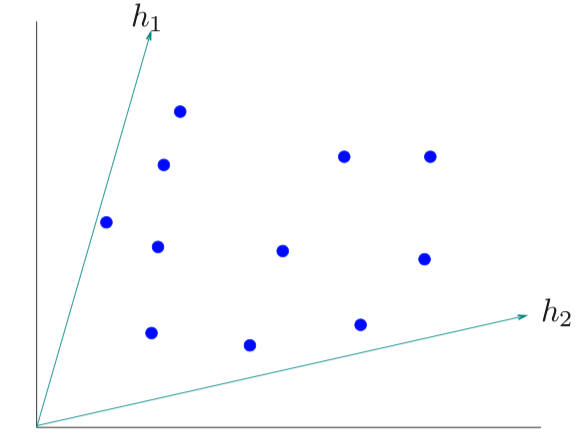
\includegraphics[scale=0.4]{img/NonUniqueness}
\caption{Any choice of the basis vectors h1 and h2 in the open space between the coordinate axes and data, gives an exact reconstruction of the data.}
\label{nonUnique}
\end{figure}

\subsubsection{Archetypal Analysis}
...

\subsection{Independent component analysis and Exploratory Projection Pursuit}
Multivariate data are often viewed as multiple indirect measurements arising from an underlying source. Variables that cannot be directly observed are called \textbf{latent variables}. Example are psychological IQ tests: answers are the multivariate variables (data) and the intelligence, is the latent variable we want to measure and that generated those data. The same for the EEG brain scans to measure neuronal activity: electromagnetic signals are measured by sensors placed at different points. Other examples exist.

\subsubsection{Latent variables and Factor analysis}
Factor analysis is a statistical technique that aims to find latent sources mostly exploiting Gaussian distributions.
Consider the SVD:
\begin{equation}
\begin{aligned}
\X &= \mathbf{UDV}^T\\
\mathbf{S} &= \sqrt{N}\mathbf{U}\\
\mathbf{A}^T = \frac{\mathbf{DV}^T}{\sqrt{N}}\\
\Rightarrow \X = \mathbf{SA}^T
\end{aligned}
\end{equation}
and hence each of the columns of $\X$ is a linear combination of the columns of $\mathbf{S}$. Now since $\mathbf{U}$ is orthogonal, and assuming as before that the columns of $\X$ (and hence $\mathbf{U}$) each have mean zero, this implies that the columns of $\mathbf{S}$ have zero mean, are uncorrelated and have unit variance.

However this representation is not unique: given the orthogonal matrix $\mathbf{R}$: $\X = \mathbf{AR^TRS}$.  It is therefore impossible to identify any particular latent variables as unique underlying sources.

With $q<p$ the classical factor analysis is $X = AS + \epsilon$. Here $\mathbf{S}$ is a vector of $q < p$ underlying latent variables or factors, $A$ is a $p \times q$ matrix of factor loadings, and the $\epsilon_j$ are uncorrelated zero-mean disturbances. The idea is that the latent variables $S_\ell$ are common sources of variation amongst the $X_j$, and account for their correlation structure, while the uncorrelated $\epsilon_j$ are unique to each $X_j$ and pick up the remaining unaccounted variation. Typically the $S_\ell$ and the $\epsilon_j$ are modeled as Gaussian random variables, and the model is fit by maximum likelihood.

The parameters all reside in the covariance matrix
\begin{equation}
\Sigma = AA^T +D_\epsilon
\end{equation}
Lack of uniqueness still remains.

\subsubsection{Independent Component analysis}
ICA assumes $S_\ell$ to be statistically independent rather than uncorrelated. Intuitively, lack of correlation determines the second-degree cross-moments (covariances) of a multivariate distribution, while in general statistical independence determines all of the cross-moments. These extra moment conditions allow us to identify the elements of $\mathbf{A}$ uniquely.

The multivariate Gaussian distribution is determined by its second moments alone. Hence identifiability problems can be avoided if we assume that the $S_\ell$ are independent and non-Gaussian.

ICA can be used to separate two mixed signals in the classical \textbf{cocktail party problem} where different microphones  $\X_j$ pick up mixtures of different independent sources $S_\ell$. ICA is able to perform \textbf{blind source separation} by exploiting independence and non-Gaussianity of the original sources.

Defining the entropy as 
\begin{equation}
H(Y) = -\int g(y) \log g(y) dy,
\end{equation}
a result in information Theory states that among all random variables with equal variance, Gaussian variables have the maximum entropy. The \textbf{mutual information $I(Y)$}  between the components of the random vector $Y$ is a natural measure of dependence:
\begin{equation}
I(Y) = \sum_{j=1}^pH(Y_j) - H(Y)
\end{equation}
where $I(Y)$ is called \textbf{Kullback-Leibler distance} between the density $g(y)$ of $Y$ and its independence version $\prod_{j=1}^p g_j(y_j)$ where $g_j(y_j)$ is the marginal density of $Y_J$.

Now if $\X$ has covariance $\I$, and $Y = A^T\X$ with $A$ orthogonal, then it is easy to show that:
\begin{equation}
\begin{aligned}
I(Y) = \sum_{j=1}^p H(Y_j)-H(X) - \log |det(A)| = \sum_{j=1}^p H(Y_j)-H(X)
\end{aligned}
\end{equation}

Finding an $A$ to minimize $I(Y)$ looks for the orthogonal transformation that leads to the most independence between its components. For convenience, rather than using the entropy $H(Y_j)$, the negentropy measure is sometimes used $J(Y_j)$ defined by:
\begin{equation}
J(Y_j) = H(Z_j) - H(Y_j)
\end{equation}
where $Z_j$ is a Gaussian random variable with the same variance as $Y_j$ . Negentropy is non-negative, and measures the departure of $Y_j$ from Gaussianity. ICA solutions use the approximation:
\begin{equation}
\begin{aligned}
J(Y_j) &\sim \left[EG(Y_j) - EG(Z_j)\right]\\
G(u) = \frac{1}{a}\log\cosh(au) \quad\quad 1\le a \le 2
\end{aligned}
\end{equation}
In summary then, ICA applied to multivariate data looks for a sequence of orthogonal projections such that the projected data look as far from Gaussian as possible.

ICA has become an important tool in the study of brain dynamics.

\subsubsection{Exploratory Projection Pursuit}
It is graphical exploration technique for visualizing high-dimensional data. It assumes projections of high-dimensional data look Gaussian. Interesting structure, such as clusters or long tails, would be revealed by non-Gaussian projections.

It proposes a number of projection indices for optimization, each focusing on a different departure from Gaussianity. Typically with projection pursuit, the directions $a_j$ are not constrained to be orthogonal.

MDS requires only the dissimilarities $d_{ij}$.

Multidimensional scaling seeks values $z_1, \cdots , z_N \in \CMcal{R}^k$ to minimize the so-called stress function:
\begin{equation}
S_M(z_1, \cdots, z_N) = \sum_{i\ne j}\br{d_{ij}- \| z_i - z_j \|}^2
\end{equation}
This is known as \textbf{least squares} or \textbf{Kruskal-Shepherd scaling}. The idea is to find a lower-dimensional representation of the data that preserves the pairwise distances as well as possible. Notice that the approximation is in terms of the distances rather than squared distances. A gradient descent algorithm is used to minimize SM.
A variation on least squares scaling is the so-called \textbf{Sammon mapping} which minimizes:
\begin{equation}
S_{S_m}(z_1, \cdots, z_N = \sum_{i\ne j}\frac{\br{d_{ij} - \|z_i - z+j\|}^2}{d_{ij}}
\end{equation}
Here more emphasis is put on preserving smaller pairwise distances.

In classical scaling, we instead start with similarities $s_{ij}$ : often we use the centred inner product $s_{ij} = \left\langle x_i - \bar{x} , x_j - \bar{x}\right\rangle$. The problem then is to minimize
\begin{equation}
S_C(z_1, \cdots, z_N) = \sum_{i,j} \br{s_{ij} - \left\langle z_i-\bar{z}, z_j - \bar{z}\right\rangle}^2
\end{equation}
This is attractive because there is an explicit solution in terms of eigenvectors. If we have Euclidean distances instead of inner products we can convert them to centred inner-products. If the similarities are in fact centred inner-products, classical scaling is exactly equivalent to principal components, an inherently linear dimension-reduction technique. Classical scaling is not equivalent to least squares scaling; the loss functions are different, and the mapping can be nonlinear.

Least squares and classical scaling are referred to as \textbf{metric scaling methods}, in the sense that the actual dissimilarities or similarities are approximated. \textbf{Shephard-Kruskal nonmetric scaling} effectively uses only ranks:
\begin{equation}
S_{NM}(z_1, \cdots, z_N)  = \frac{\sum_{i\ne j} \left[ \|z_i - z_j\| - \theta(d_{ij})\right]^2}{\sum_{i\ne j}\|z_i - z_j\| }
\end{equation}
over $z_i$ and an arbitrary increasing function $\theta$. With $\theta$ fixed, we minimize over $z_i$ by gradient descent. With the $z_i$ fixed, the method of isotonic regression is used to find the best monotonic approximation $\theta(d_{ij})$ to $\|z_i - z_j \|$. These steps are iterated until the solutions stabilize.